\documentclass[11pt,a4paper]{article}

\usepackage[a4paper,margin=2.2cm]{geometry}
\usepackage{fontspec}
\usepackage{graphicx}
\usepackage{xcolor}
\usepackage{booktabs}
\usepackage{longtable}
\usepackage{array}
\usepackage{enumitem}
\usepackage{listings}
\usepackage{tcolorbox}
\usepackage{fancyhdr}
\usepackage{titlesec}
\usepackage{microtype}
\usepackage[colorlinks=true,linkcolor=lloydsblue,urlcolor=lloydsblue,citecolor=lloydsblue]{hyperref}

\definecolor{lloydsblue}{HTML}{0C3B6E}
\definecolor{lloydsgreen}{HTML}{1F7A4D}
\definecolor{codebg}{HTML}{F4F6FA}
\definecolor{notebg}{HTML}{EEF3FB}

\titleformat{\section}{\Large\bfseries\color{lloydsblue}}{\thesection}{0.6em}{}
\titleformat{\subsection}{\large\bfseries\color{lloydsblue}}{\thesubsection}{0.6em}{}

\lstset{
  basicstyle=\ttfamily\small,
  backgroundcolor=\color{codebg},
  frame=single,
  rulecolor=\color{lloydsblue!40},
  breaklines=true,
  showstringspaces=false,
  columns=fullflexible,
  xleftmargin=4pt,
  xrightmargin=4pt
}

\newtcolorbox{note}[1][]{
  colback=notebg, colframe=lloydsblue!60, boxrule=0.6pt,
  arc=2pt, left=6pt, right=6pt, top=4pt, bottom=4pt, #1
}

\pagestyle{fancy}
\fancyhf{}
\fancyhead[L]{\small\color{lloydsblue}Copilot Usage Logger --- Technical Document}
\fancyhead[R]{\small\color{lloydsblue}v0.11.0}
\fancyfoot[C]{\small\thepage}
\renewcommand{\headrulewidth}{0.6pt}
\renewcommand{\footrulewidth}{0pt}

\newcommand{\code}[1]{\texttt{\color{lloydsblue!80!black}#1}}

\title{\color{lloydsblue}\textbf{Technical Document}\\[4pt]\Large Copilot Usage Logger}
\author{Lloyds Banking Group --- Developer Experience}
\date{Version 0.11.0}

\begin{document}
\sloppy
\maketitle
\thispagestyle{fancy}

\begin{note}
\textbf{Audience:} engineers maintaining or extending this extension.
\end{note}

\tableofcontents
\newpage

\section{Purpose}

VS Code extension that locally logs, classifies, and reports on a
developer's GitHub Copilot Chat usage (requests, cost units/``credits'',
categories, languages, models), with no data leaving the machine unless
company-wide reporting is explicitly enabled. It also exposes optional
read-only ``knowledge grounding'' chat tools (Confluence, Jira, GitHub,
SharePoint, Teams) and a local ``who to contact'' skill (\code{find\_help})
so Copilot chat can cite internal documentation/issues/code and route
non-code blockers to the right owner.

\section{Why This Exists (Design Constraints)}

There is no public VS Code API to observe requests sent to the built-in
\code{@copilot} participant --- chat participants only see turns explicitly
@-mentioned to them. VS Code Copilot Chat does, however, persist full
conversation history to local JSON files under the user's VS Code profile.
This extension watches and parses those files. The on-disk format is
\textbf{undocumented and internal} and may change across VS Code versions
without notice, so every parse entry point is defensive (catches and skips
malformed entries, records \code{schema\_version\_seen} and error counts per
file rather than throwing).

Two independent capture paths exist and are deliberately deduplicated:

\begin{itemize}[leftmargin=1.4em]
  \item \textbf{Passive}: a file watcher + parser over VS Code's own chat
  session files (primary, automatic, broad coverage).
  \item \textbf{Participant}: a custom \code{@usage} chat participant
  (secondary, explicit, fully controlled). Its own turns land in the same
  session files as normal chat, so the ingestor skips entries whose
  \code{agent.id} matches the extension's own participant id to avoid
  double-counting.
\end{itemize}

\section{High-Level Architecture}

\begin{figure}[h!]
  \centering
  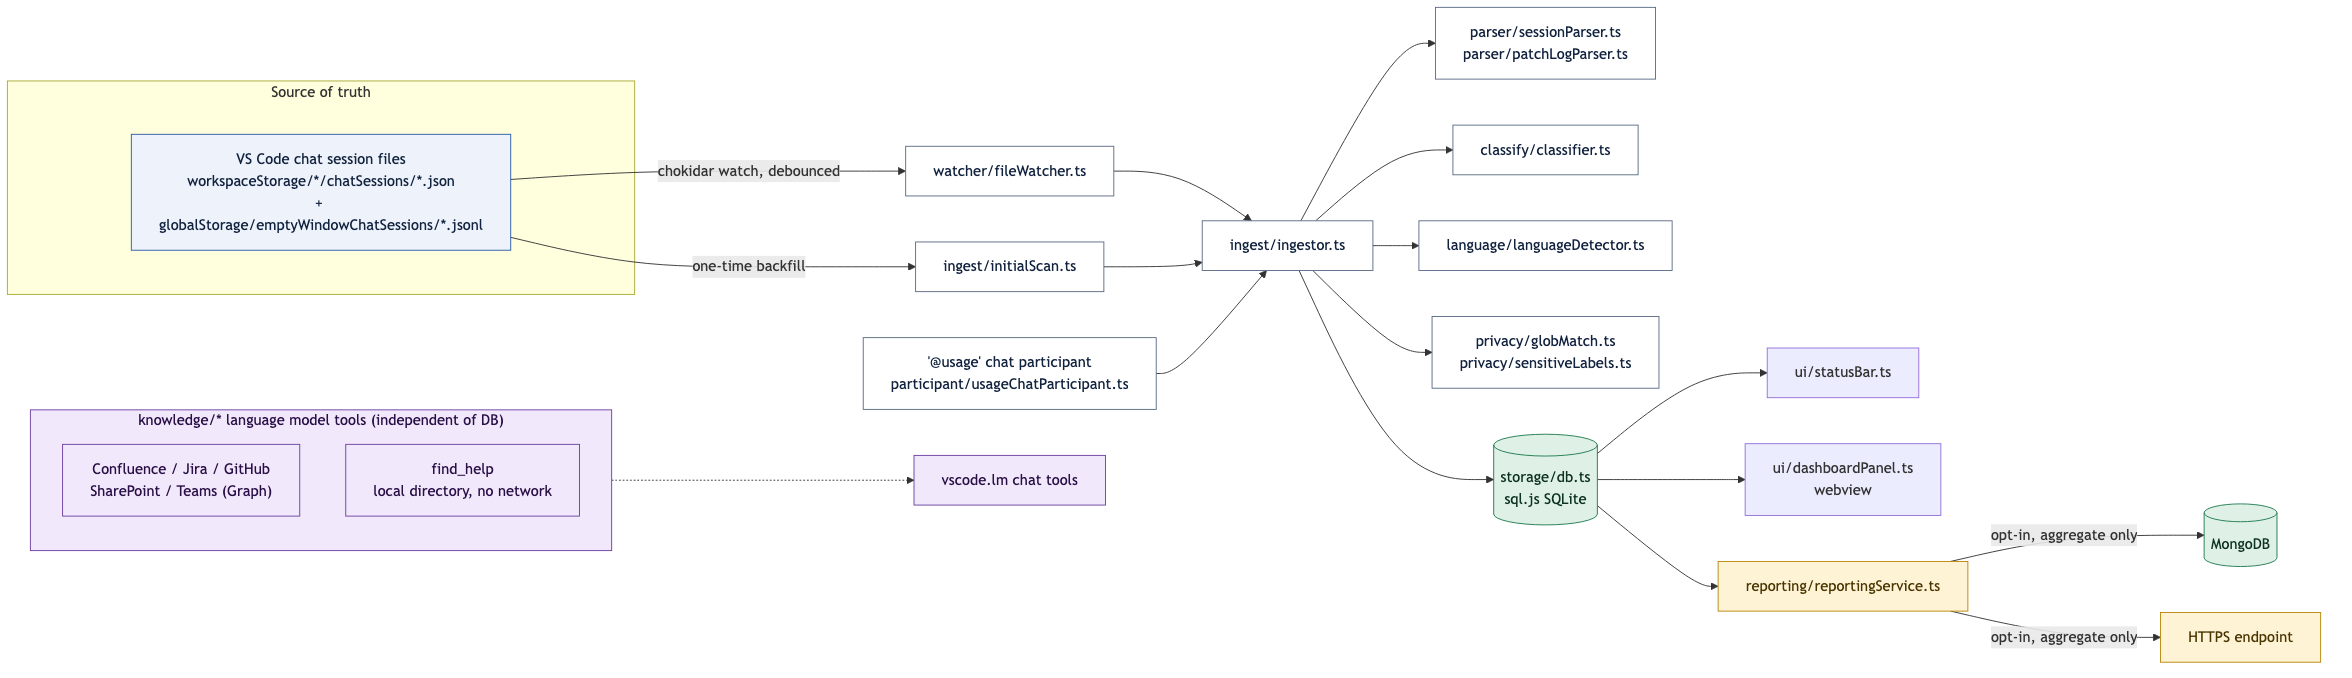
\includegraphics[width=\textwidth]{media/architecture-diagram.png}
  \caption{Data flow from VS Code's chat session files through ingestion to
  storage, UI, optional company-wide reporting, and the independent
  knowledge-tool layer.}
\end{figure}

\section{Module Map (\texttt{src/})}

Grouped by subsystem --- see the source tree for individual file names.

\begin{longtable}{@{}p{4.2cm}p{10.8cm}@{}}
\toprule
\textbf{Subsystem} & \textbf{Responsibility} \\
\midrule
\endhead
\code{extension.ts} & Activation entry point: wires every subsystem below, registers commands and config-change listeners. \\
\code{discovery/}, \code{watcher/} & Locates both chat-log roots (workspace-scoped and global empty-window) and watches them with chokidar (\code{awaitWriteFinish} debounce). \\
\code{parser/} & Defensive parsers for both undocumented VS Code chat-log formats (workspace snapshot, empty-window patch-log); never throw. \\
\code{classify/}, \code{language/} & Buckets each request into a category (debug, refactor, test, docs, \ldots) and detects its primary language. \\
\code{privacy/} & Path-glob exclusion and sensitive-keyword redaction --- applied before anything is written. \\
\code{storage/} & sql.js SQLite schema/migrations, idempotent inserts, all aggregate queries. \\
\code{ingest/} & Ties parse $\rightarrow$ privacy filter $\rightarrow$ classify $\rightarrow$ store together; per-file cursors plus a one-time backfill scan. \\
\code{participant/} & \code{@usage} chat participant (\code{/stats} slash command). \\
\code{ui/} & Status bar item and the dashboard webview. \\
\code{reporting/} & Optional opt-in company-wide aggregate reporting: HTTPS/MongoDB transport, device id, multi-device credit sync. \\
\code{heuristics/} & Dashboard heuristics --- model-fit suggestions, estimated time saved per category. \\
\code{export/} & CSV export of logged requests for audit. \\
\code{knowledge/} & Read-only language model tools: Confluence, Jira, GitHub, SharePoint/Teams (Graph), and \code{find\_help} (fully local). \\
\bottomrule
\end{longtable}

\begin{note}
Pure logic used by unit tests (classifier, language detector, glob matching,
model fit, time savings, and all \code{*Text.ts} knowledge-tool formatters)
is kept in files with no \code{vscode} import, since vitest cannot import
the \code{vscode} module. Vscode-coupled orchestration stays in adjacent
files.
\end{note}

\section{Storage Schema (sql.js / SQLite)}

\begin{lstlisting}[language=SQL]
CREATE TABLE requests (
  id INTEGER PRIMARY KEY AUTOINCREMENT,
  session_id TEXT, request_id TEXT,
  source TEXT CHECK(source IN ('passive','participant')),
  workspace_hash TEXT, workspace_path TEXT,
  timestamp INTEGER,               -- original request time, epoch ms
  category TEXT,                   -- free text, tunable without migration
  language TEXT,
  model_id TEXT,
  agent_id TEXT, agent_name TEXT,
  prompt_text TEXT,
  response_text TEXT,
  attachments_json TEXT,
  copilot_credits REAL,
  schema_version_seen INTEGER,
  created_at INTEGER,
  UNIQUE(session_id, request_id, source)
);
-- indexes on timestamp, category, language

CREATE TABLE ingestion_state (
  file_path TEXT PRIMARY KEY,
  last_mtime_ms INTEGER, last_size_bytes INTEGER, last_request_count INTEGER,
  last_processed_at INTEGER, schema_version_seen INTEGER,
  parse_error_count INTEGER, last_error TEXT
);
\end{lstlisting}

\code{UNIQUE(session\_id, request\_id, source)} plus per-file cursors in
\code{ingestion\_state} make re-ingestion idempotent: only new/changed
requests are parsed on each pass. \code{SCHEMA\_USER\_VERSION} (currently 3)
is applied via \code{PRAGMA user\_version} migrations in
\code{storage/schema.ts}.

\begin{note}
\textbf{Storage location:} \code{context.globalStorageUri}, not
\code{context.storageUri}, because source data spans many workspaces plus
global empty-window sessions, and \code{context.storageUri} is
\code{undefined} with no folder open. sql.js is in-memory-first WASM
SQLite --- the DB is \code{export()}ed to bytes and written to disk on a
debounced idle timer and in \code{deactivate()}; rows written between
flushes can be lost on a crash (accepted trade-off, no WAL).
\end{note}

\section{Data Flow (Single Request, Passive Path)}

\begin{enumerate}[leftmargin=1.6em]
  \item User sends a Copilot Chat message $\rightarrow$ VS Code writes/updates a \code{chatSessions/<id>.json} file.
  \item chokidar (debounced via \code{awaitWriteFinish}) fires a change event.
  \item \code{ingestor.ts} re-parses the file via \code{sessionParser.ts}, using the file's \code{ingestion\_state} cursor to only look at new/changed requests.
  \item Each new request is checked against \code{usageLogger.excludedPathGlobs} (dropped entirely if matched) and against the extension's own participant \code{agent.id} (dropped if it's \code{@usage}'s own turn).
  \item Remaining requests are classified, language is detected, and the row is upserted into \code{requests} (idempotent on the \code{UNIQUE} constraint).
  \item \code{statusBar.ts} and any open \code{dashboardPanel.ts} are refreshed.
  \item If \code{usageLogger.enableCompanyWideReporting} is on, \code{reportingService.ts} periodically ships aggregate payloads to the configured HTTPS endpoint or MongoDB collection.
\end{enumerate}

\section{Status Bar}

\code{ui/statusBar.ts} shows, per \code{usageLogger.statusBarDisplay}:

\begin{itemize}[leftmargin=1.4em]
  \item \code{"requests"} (default): today's request count, \code{\$(copilot) \{n\} today}.
  \item \code{"remainingCredits"}: remaining cost-unit budget for today, computed from \code{dailyBudgetInfo()}. Falls back to the request-count display if \code{usageLogger.monthlyCreditLimit} isn't set.
  \item Private mode: lock icon, logging paused.
  \item Amber background/warning icon once today's spend meets/exceeds today's even daily-budget share, in either display mode.
\end{itemize}

The setting is read live in \code{refresh()} (no cached field), and
\code{extension.ts}'s \code{onDidChangeConfiguration} listener calls
\code{statusBar.refresh()} on change so toggling it takes effect
immediately, no reload required.

\section{Dashboard Webview}

\code{ui/dashboardPanel.ts} hosts a \code{WebviewPanel} with inline
HTML/CSS/JS (no charting library --- hand-built SVG). \code{postData()}
sends: counts by category/language/model/day, \code{creditsByModel()},
\code{creditsByDay()}, \code{projectedMonthEnd} (burn-rate forecast),
model-fit and time-savings heuristics, and multi-device credit sync state.
A parallel \code{companyDashboardPanel.ts} renders aggregate data reported
by other devices when company-wide reporting is enabled.

\section{Knowledge Tools (Confluence / Jira / GitHub / Graph / Find-Help)}

Independent of the usage-tracking DB. Each is a read-only
\code{vscode.lm.registerTool} implementation registered via
\code{contributes.languageModelTools} (requires \code{engines.vscode >= 1.95}).

\begin{longtable}{@{}p{3.6cm}p{6.2cm}p{5.2cm}@{}}
\toprule
\textbf{Tool} & \textbf{Source} & \textbf{Auth} \\
\midrule
\endhead
\code{search\_confluence}, \code{get\_confluence\_page} & Confluence Cloud REST API & Atlassian email + API token (Basic auth) \\
\code{search\_jira}, \code{get\_jira\_issue} & Jira Cloud REST API & Same Atlassian email + API token as Confluence \\
\code{search\_github} & GitHub REST/code search API & Personal access token, \code{Authorization: Bearer} \\
\code{search\_sharepoint}, \code{search\_teams} & Microsoft Graph \code{/search/query} & Delegated access token, \code{Authorization: Bearer} --- short-lived (~1h), no refresh flow \\
\code{find\_help} & Local JSON ``blocker directory'' & None --- no network, no credentials \\
\bottomrule
\end{longtable}

Security posture (applies to the network-backed tools): HTTPS-only
(\code{httpJson.ts} refuses \code{http://}), 5MB response cap, 10s default
timeout, tokens stored in \code{context.secrets} (never in settings.json,
never logged), read-only operations only, and results are bounded by the
underlying service's own permissions.

\code{find\_help} is the exception to the network posture: it makes
\textbf{no} outbound calls at all. It matches the free-text blocker against
a local directory (\code{blockerText.ts}, pure/unit-tested scoring), loaded
by \code{blockerRoutes.ts} from \code{usageLogger.blockerDirectory} (inline),
then \code{usageLogger.blockerDirectoryPath} (a JSON file), falling back to
the bundled \code{media/blocker-directory.sample.json}.
\code{parseBlockerDirectory} drops any link whose scheme isn't in an
allowlist (\code{https}/\code{http}/\code{msteams}/\code{mailto}), so a
malicious directory can't smuggle a \code{javascript:}/\code{file:} link
into a rendered suggestion.

\section{Configuration Surface (\texttt{contributes.configuration})}

Key settings (see \code{package.json} for the authoritative list/defaults):
\code{enablePassiveCapture}, \code{retentionDays}, \code{privateMode},
\code{excludedPathGlobs}, \code{sensitiveLabelKeywords},
\code{monthlyCreditLimit}, \code{statusBarDisplay},
\code{timeSavingsMinutesPerCategory}, \code{enableCompanyWideReporting},
\code{reportingEndpointUrl}, \code{reportingIntervalMinutes},
\code{reportingTransport}, \code{allowInsecureHttp}, \code{mongoDatabase},
\code{mongoCollection}, \code{confluenceBaseUrl}, \code{confluenceEmail},
\code{atlassianEmail}, \code{jiraBaseUrl}, \code{githubOrg},
\code{blockerDirectoryPath}, \code{blockerDirectory}.

Commands (Command Palette, prefix \code{Copilot Usage:}): Open Dashboard,
Open Company-Wide Dashboard, Rescan Chat History, Purge All Logged Data,
Send Company-Wide Report Now, Set/Clear Reporting API Key, Set/Clear
MongoDB Connection String, Toggle Private Mode, Export Audit CSV, Sync
Actual Credits Used This Month, Set/Clear Confluence API Token, Test
Confluence Connection, Test Jira Connection, Set/Clear GitHub Token, Open
Help Directory, Setup (guided walkthrough entry point).

\section{Security Posture (OWASP-Relevant)}

\begin{itemize}[leftmargin=1.4em]
  \item \textbf{No secrets in settings.json}: API tokens (Confluence/Jira, GitHub, Mongo connection string, reporting API key) live in \code{context.secrets} (VS Code SecretStorage), not workspace/user settings.
  \item \textbf{Transport security}: all outbound HTTP requires HTTPS by default; plaintext HTTP requires explicitly opting in via \code{usageLogger.allowInsecureHttp}.
  \item \textbf{Bounded I/O}: knowledge-tool responses are capped at 5MB and a 10s timeout to avoid unbounded memory/hangs from a compromised or slow upstream.
  \item \textbf{Least privilege}: all knowledge tools are read-only and respect the underlying service's existing permissions --- no writes, no privilege escalation.
  \item \textbf{Local-first data}: full prompt/response text is stored unencrypted under \code{context.globalStorageUri}; called out prominently in \code{README.md}. Mitigations: \code{retentionDays}, \code{purgeData} command, \code{privateMode}, \code{excludedPathGlobs}.
  \item \textbf{Idempotent ingestion}: \code{UNIQUE(session\_id, request\_id, source)} plus per-file cursors prevent duplicate/replayed rows from a re-triggered watcher event.
  \item \textbf{Defensive parsing}: the chat session file format is undocumented and can change; parsers catch and skip malformed entries per-request rather than throwing, and track \code{schema\_version\_seen}/error counts for diagnosis.
  \item \textbf{Safe link handling}: \code{find\_help}'s directory parser allowlists only \code{https}/\code{http}/\code{msteams}/\code{mailto} link schemes before rendering them.
\end{itemize}

\section{Build, Test, and Release}

\begin{itemize}[leftmargin=1.4em]
  \item Type-check: \code{npx tsc --noEmit}
  \item Unit tests: \code{npx vitest run} (88 tests across 12+ files; only vscode-free modules are covered)
  \item Lint: \code{npx eslint src}
  \item Dev bundle: \code{node esbuild.js}; production bundle: \code{node esbuild.js --production} (a custom plugin copies \code{sql-wasm.wasm} into \code{dist/})
  \item Package: \code{rm -f *.vsix \&\& npx @vscode/vsce package --no-dependencies --allow-star-activation}
  \item Local install: install via the VS Code CLI \code{--install-extension}, then remove the previous version's extension directory
  \item Release: commit $\rightarrow$ \code{git tag vX.Y.Z} $\rightarrow$ push branch and tag $\rightarrow$ GitHub Actions ``CI'' and ``Release'' workflows build/test and attach the \code{.vsix} to a GitHub Release.
\end{itemize}

\section{Known Limitations / Deferred Scope}

\begin{itemize}[leftmargin=1.4em]
  \item No public VS Code/GitHub API exposes org-level Copilot premium-request quota to third-party extensions; cross-device totals rely on the manual \code{creditsSync.ts} reconciliation flow rather than a live API.
  \item Remote windows (SSH/WSL/Codespaces): \code{context.globalStorageUri} resolves remote-side and may not reflect local chat activity; not a primary target.
  \item Chat session file format is internal/undocumented and may change across VS Code versions without notice.
\end{itemize}

\end{document}
